\documentclass{article}
\usepackage[utf8]{inputenc}
\usepackage{geometry} 
\geometry{a4paper}
\usepackage{wrapfig} 
\usepackage{graphicx} % support the \includegraphics command and options
\usepackage{subfigure}
\usepackage{booktabs} % for much better looking tables
\usepackage{array} % for better arrays (eg matrices) in maths
\usepackage{paralist}
\usepackage{subfig}
\usepackage{verbatim}
\usepackage{appendix}
\usepackage{fancyhdr}
\usepackage{sectsty}
\usepackage[dvipsnames,svgnames]{xcolor}
\usepackage{amsmath}
\usepackage[format=plain,
            font=it]{caption} % Italicizes figure captions
\usepackage[english]{babel}
\usepackage[nottoc,notlof,notlot]{tocbibind} % Put the bibliography in the ToC
\usepackage[titles,subfigure]{tocloft} % Alter the style of the Table of Contents
\renewcommand{\cftsecfont}{\rmfamily\mdseries\upshape}
\renewcommand{\cftsecpagefont}{\rmfamily\mdseries\upshape} % No bold!

\usepackage{imakeidx}
\usepackage{csquotes}
\usepackage{graphicx} % Allows you to insert figures
\usepackage{amsmath} % Allows you to do equations
\usepackage{fancyhdr} % Formats the header
\usepackage{geometry} % Formats the paper size, orientation, and margins
\linespread{1.25} % about 1.5 spacing in Word
\setlength{\parindent}{0pt} % no paragraph indents
\setlength{\parskip}{1em} % paragraphs separated by one line
\usepackage[style=authoryear-ibid,backend=biber,maxbibnames=99,maxcitenames=2,uniquelist=false,isbn=false,url=true,eprint=false,doi=true,giveninits=true,uniquename=init]{biblatex} % Allows you to do citations - does Harvard style and compatible with Zotero
\urlstyle{same} % makes a nicer URL and DOI font 
\AtEveryBibitem{
    \clearfield{urlyear}
    \clearfield{urlmonth}
} % removes access date
\AtEveryBibitem{\clearfield{month}} % removes months in bibliography
\AtEveryCitekey{\clearfield{month}} % removes months in citations
\renewbibmacro{in:}{} % Removes the "In" before journal names

\renewbibmacro*{editorstrg}{%from biblatex.def
  \printtext[editortype]{%
    \iffieldundef{editortype}
      {\ifboolexpr{
         test {\ifnumgreater{\value{editor}}{1}}
         or
         test {\ifandothers{editor}}
       }
         {\bibcpstring{editors}}
         {\bibcpstring{editor}}}
      {\ifbibxstring{\thefield{editortype}}
         {\ifboolexpr{
            test {\ifnumgreater{\value{editor}}{1}}
            or
            test {\ifandothers{editor}}
          }
            {\bibcpstring{\thefield{editortype}s}}%changed
            {\bibcpstring{\thefield{editortype}}}}%changed
         {\thefield{editortype}}}}}

\renewbibmacro*{byeditor+others}{%from biblatex.def
  \ifnameundef{editor}
    {}
    {\printnames[byeditor]{editor}%
     \addspace%added
     \mkbibparens{\usebibmacro{editorstrg}}%added
     \clearname{editor}%
     \newunit}%
  \usebibmacro{byeditorx}%
  \usebibmacro{bytranslator+others}}
  % The commands above from lines 20-49 change the way editors are displayed in books
\AtEveryBibitem{%
  \clearlist{language}%
} % removes language from bibliography
\citetrackerfalse 
% Removes ibids (ibidems)
\DeclareNameAlias{sortname}{family-given} % Ensures the names of the authors after the first author are in the correct order in the bibliography
\renewcommand*{\revsdnamepunct}{} % Corrects punctuation for authors with just a first initial
\addbibresource{Example.bib} % Tells LaTeX where the citations are coming from. This is imported from Zotero
\usepackage[format=plain,
            font=it]{caption} % Italicizes figure captions
\usepackage[english]{babel}
\usepackage{csquotes}
\renewcommand*{\nameyeardelim}{\addcomma\space} % Adds comma in in-text citations
\renewcommand{\headrulewidth}{0pt}
\geometry{letterpaper, portrait, margin=1in}
\setlength{\headheight}{14.49998pt}

\newcommand\titleofdoc{Turbolent diffusion of Fe in Perseus cluster} %%%%% Put your document title in this argument
\newcommand\GroupName{Students names} %%%%% Put your group name here. If you are the only member of the group, just put your name

\begin{document}
\begin{titlepage}
   \begin{center}
        \vspace*{4cm} % Adjust spacings to ensure the title page is generally filled with text

        \Huge{\titleofdoc} 

        \vspace{0.5cm}
        \LARGE{project 2}
            
        \vspace{3 cm}
        \Large{\GroupName}
       
        \vspace{0.25cm}
        \large{Teresa Zorzi, Chiara Zerbinati,Matteo Sapori}
       
        \vspace{3 cm}
        \Large{July 25, 2022}
        
        \vspace{0.25 cm}
        \Large{Computational for physics and astrophysics}
       

       \vfill
    \end{center}
\end{titlepage}

\setcounter{page}{2}
\pagestyle{fancy}
\fancyhf{}
\rhead{\thepage}
\lhead{\GroupName; \titleofdoc}



%___________________________________________________________



%%% HEADERS & FOOTERS
 % This should be set AFTER setting up the page geometry
\pagestyle{fancy} % options: empty , plain , fancy
\renewcommand{\headrulewidth}{0pt} % customise the layout...
\lhead{}\chead{}\rhead{}
\lfoot{}\cfoot{\thepage}\rfoot{}

%%% SECTION TITLE APPEARANCE

\allsectionsfont{\sffamily\mdseries\upshape} % (See the fntguide.pdf for font help)
% (This matches ConTeXt defaults)

%%% ToC (table of contents) APPEARANCE

%%% END Article customizations

%%% The "real" document content comes below...


%\date{} % Activate to display a given date or no date (if empty),
         % otherwise the current date is printed 


\tableofcontents
\newpage

%_________________________________________________________________________________________gg
\section{Introduction}
\subsection{Brief astrophysical background}
Clusters of galaxies are gravitationally bound aggregations of
galaxies containing hundreds to thousands of galaxies. The most regular clusters are believed to be almost virialized, i.e. close to dynamical equilibrium.\\
Most of the mass in clusters (\(84-90\% )\) is in the form of dark matter, while only \(10–16\%\) of the mass is in the form of baryons, mostly hot gas. \\
The most luminous galaxy in a cluster is called the brightest cluster galaxy (BCG), and it's invariably a giant elliptical. The BCGs, which typically sit at the center of their clusters, are the most luminous galaxies in the Universe, with luminosities up to \(10^{12}\;L_{\odot}\). \\
The ISM of these galaxies has been processed by a large amount of SN Ia: each SN injects about  \(10^{51} \; erg\) and metals in the ICM, especially Fe.\\ By the theory of galaxies formation, massive elliptical must have formed most of their stellar mass in a very short time know as starburst: during a starburst event a lot of massive stars are created; those stars are the progenitors that will eventually generate the supernovas that will enrich the galaxy ISM. After that, due to external pressure inside the cluster, part of this gas will be stripped from the galaxy to become part of the intra-cluster medium.\\ Even though the internal dynamic of ICM is a tough subject, most of the metals present in the gas get spread in the ICM via turbulent diffusion.

\subsection{Aim of the project}
Since SNe largely contribute to the enrichment of the ICM, we want to estimate the amount of metals ejected and their spatial distribution.\\
However, observations show that the iron distribution in clusters is much more extended than the central galaxy, suggesting that some mechanism is spreading iron up to larger scales.\\
Most studies assume that some turbulence is mixing the gas and diffusing metals outwards: we want to study this problem.


\section{Preparation of the problem}
\subsection{Gas distribution in the Cluster}

As the first step, we want to estimate the gas distribution in the cluster. We assume it to be in equilibrium; so, its behavior is regulated by the hydrostatic equilibrium equation:

\begin{equation} \frac{dP}{dr}=-\frac{GM(<r)}{r^{2}}\rho \end{equation}

However, the mass term in eq 1 does not account for only barions, but for all mass present that generates gravity; dark matter included.\\ 
Since the cluster's halo is dominated by dark matter, we need to set its density profile. As a theoretical model, we will consider the \textbf{Navarro-Frank-White} profile:

\begin{equation}
\rho_{DM}(r)=\frac{\rho_{DM,0}}{\frac{r}{r_{s}}(1-\frac{r}{r_{s}})}.\label{eq:dmdensity}
\end{equation}

Here, \(\rho_{DM,0}\) and \(r_{s}\) depend on the cluster mass, which in our case is \(M_{virial}\sim M_{DM}\sim 1.2 \times 10^{15}M_{\odot}\), giving:

\vspace{-10 mm}
\begin{center}
\begin{align*}
\rho_{DM,0}=7.35\times 10^{-26}\; g/cm^{3}\qquad r_{s}=435.7\;kpc.\
\end{align*}
\end{center}
\vspace{2 mm}

The virial radius of the cluster is \(r_{vir}\sim 2.8 \;Mpc\).\\
From the DM density profile ( eq \ref{eq:dmdensity}), the mass profile can be computed analitically :

\begin{equation}
M_{DM}(r)=\int_{0}^{r}\rho_{DM}(r)dV=\int_{0}^{r}4\pi r^{2}\rho_{DM}(r)dr.
\end{equation}

Notice that spherical symmetry is assumed.\\
We will compute the mass profile numerically: the construction of the grid will be illustrated in the following section.

\subsection{The Grid}
Like as in project 1, we will solve finite-differences-equations, so we replace the continuum with a grid of points, setting as extremes: \(r_{min}=0\;Mpc\) and \(r_{max}=3\;Mpc\). \\ 
In order to properly center the variables, the grid is constructed as the sum of two decentralized grids (\textit{r} and \textit{rr}) such that:

\begin{center}

$r-rr = 0.5 \cdot \Delta r$ \\
${r}_{j+1/2}=rr_{j}=\frac{1}{2}(r_j+r_{j+1})$
\end{center}


We set the number of points in each grid to be 500 thus making them separated by:

\begin{center}
$\Delta r = r(j+1)-r(j)= rr(j+1) - rr(j) = 0.5 $ $Mpc$. 
\end {center}

The volume between two adjacent shells is:
\begin{equation}
	{\Delta V}_{j+1/2}=\frac{4}{3}(r_{j+1}^{3}-r_j^{3})
\end{equation}


\begin{figure}[h!]
\centering
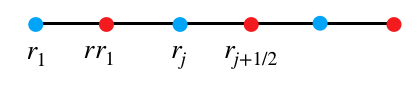
\includegraphics[width=0.5\textwidth]{griglia}
\caption{a brief scheme of the grid}
\label{fig:griglia}
\end{figure}

\newpage
\subsection{Boundary conditions}

Boundary conditions (B.C.) are implemented through a subroutine.\\
For the project, we use \textit{reflecting B.C.}, such that:

\begin{align*}
    Val(j_{min}) = Val(j_{min}+1) \\
    Val(j_{max}) = Val(j_{max}-1)
\end{align*}
Where \textit{Val} indicates the value of the generic variable for which we set the boundary conditions.

\newpage
\subsection{Dark Matter and stars mass profile}

Now we want to compare the DM mass profile analytical solution with the numerical one.
Numerically, the profile is obtained as the sum over the individual shells for each radius; the DM mass contained in a shell of thickness $ r_{(j+1/2)} -r_j$ is:
\[
    \Delta {M}_{DM,j+1/2}=\rho_{DM,j+1/2}{\Delta V}_{j+1/2}=\rho_{DM,j+1/2}\frac{4}{3}\pi({r}_{j+1}^{3}-{r}_{j}^{3}).
\]

The analytical solution is given by:

\begin{equation}
    M_{DM}(r)=4\pi\rho_{DM,0}{r_s}^3\biggl[ln\bigg(1+\frac{r}{r_s}\bigg)-\frac{r}{r+r_s}\biggl]
\end{equation}

The comparison between the numerical solution and the analytical one is represented in Figure \ref{fig:figure 1}, which shows that the solutions are approximately coincident.\\
For the stellar mass profile we used the Herquist profile (we will better introduce it in section 2.6). Again it's plotted in figure 2 alongside the dark matter mass profiles.
\begin{figure}[h]
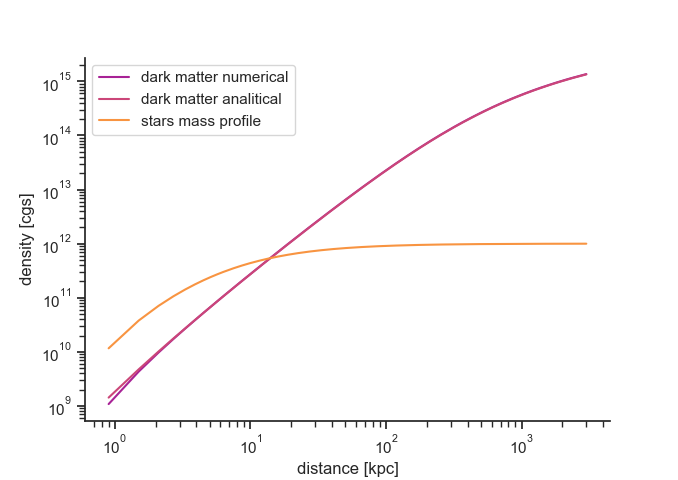
\includegraphics[width= 14 cm, trim = 0 0 0 0]{mass_profile.png}
\caption{Numerical vs Analytical solution for the DM mass}
\label{fig:figure 1}
\end{figure}

\newpage
\subsection{Hydrostatic equilibrium equation}

Once computed \(M_{DM}(r),\) we can integrate the hydrostatic equilibrium equation:

\begin{equation}
    \frac{dP}{dr}=-\frac{GM(<r)}{r^{2}}\rho_{g},
\end{equation}
 assuming the isothermal gas conditions: $ P=\frac{K\rho_{g}T}{\mu m_{p}}, $ where $ K=1.38\times 10^{-16}, \; \mu=0.61$.\\ 
 The resulting equation is:

\begin{equation}
    \frac{dln\rho_{g}}{dr}=-\frac{GM(<r)}{r^{2}}\frac{\mu m_{p}}{KT}.
\end{equation}

In order to solve the equation, we need the initial condition $\rho_{g}(0)$, which is chosen assuming the baryon fraction (eq 8), to be around \(0.16\) (cosmological value) at the virial radius of the cluster.\\ 

\begin{equation}
f_{b}=\frac{M_b}{M_{tot}}=\frac{M_{*}(r)+M_{g}(r)}{M_{*}(r)+M_{g}(r)+M_{DM}(r)}
\end{equation}

In our case, we obtained \(\rho_{0}=4.32\cdot 10^{-26}\; g/cm^{3}\). This values, actually, is grid-dependent, in order to not have to adjust this value each time the grid is modified, the code execute an "\textit{if}" cycle requiring the $f_{b}$ value not to exceed $0.17$ at the virial radius, corresponding to $2490\; kpc.$ \\
Writing now \(\rho_{g}=\rho\), the above PDE transforms into the following FDE:

\begin{equation}
    \frac{dln\rho}{dr} \rightarrow -\frac{ln\rho_{j+1/2}-ln\rho_{j-1/2}}{r_{j+1/2}-r_{j-1/2}},
\end{equation}

where the derivative is centered in \(r_{j}\). So, the equation to solve for \(\rho\) is:

\begin{equation}
    {ln\rho_{j+1/2}=-ln\rho_{j-1/2}-\Delta r \frac{GM_{j}}{r_{j}^{2}}\frac{\mu m_{p}}{kT}}
\end{equation}


Integrating the hydrostatic equilibrium equation, we can compare it with the following analytical expression for the density:
\begin{equation}\rho(r)=\rho_{0}\exp \left\{  -\frac{27}{2}b\left[1-\frac{\ln(1+r/r_{s})}{r/r_{s}}\right]\right\} =\rho_{0}e ^{-27b/2} \left(1+\frac{r}{r_{s}}\right)^{27b/(2r/r_{s})},\end{equation}
with \(b=\frac{8 \pi G\mu m_{p}\rho_{dm,0}r_{s}^{2}}{27kT}\) , which we verified to be consistent with the numerical result. The solution will give us the \textbf{isothermal gas density profile}.\\

\newpage
\subsection{Adding the BCG}
Now we have to take into account the more realistic case of the presence of a BCG: in this framework, we assume the stars to be following a "Hernquist profile" of the kind:

\begin{equation}
M_{*}(r)=M_{BCG}\frac{r^{2}}{(r+a)^2},
\end{equation}

where \(M_{BCG}=10^{12}M_{\odot}\) is the total stellar mass of the central galaxy, and $a \approx 12 $kpc. Now we have to write the new expression for \(M_{*}\) in the calculation of \(f_{g}\). 
The new initial condition for \(\rho_{0}\), obtained in the same way as before, returns: \(\rho_{0}=8.5\cdot 10^{-26}\;g/cm^{3}\).
The reason why the initial density changes, is that the BCG adds extra gravity, steepening the density profile in the central region; the effect is represented in Figure \ref{fig:figure2}.

\begin{figure}[hb]
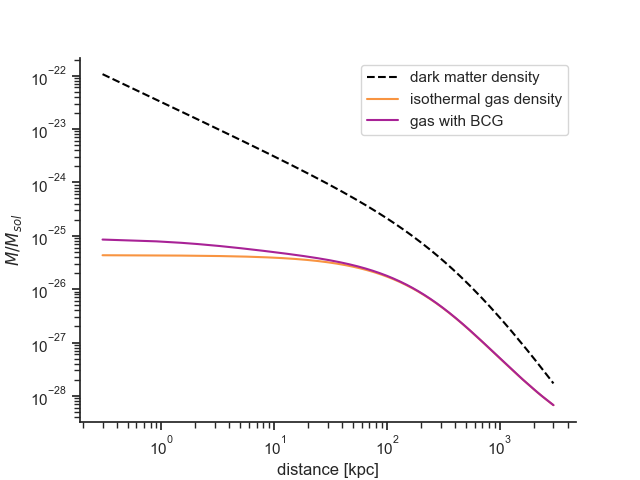
\includegraphics[width=0.8\textwidth]{gas2.png}
\caption{Comparison between the density profiles in presence and without the BCG}
\label{fig:figure2}
\end{figure}

\newpage
\subsection{Considering a more realistic T profile}
As last step, we will consider a temperature profile that is no more isothermal:

\begin{equation}
\frac{T(r)}{T_{mg}}=1.35\frac{(x/0.045)^{1.9}+0.45}{(x/0.045)^{1.9}+1}\frac{1}{1+(x/0.6)^{2})^{0.45}},
\end{equation}

where \(T_{mg}=8.9\cdot 10^{7}\;K\), and  \(x=(r/r_{500}),\) with \(r_{500}\sim r_{vir}/2=1.4 \; Mpc\).
The comparison with the isothermal profile is provided in Figure \ref{fig:figure3}.\\Now we compute again the new value of the initial density, obtaining \(\rho_{0}=1.489 \cdot 10^{-25}\; g/cm^{3}\). Again, we show the comparison between the density with an isothermal profile and no BCG, and the one taking into account the BCG and the non isothermal profile in Figure \ref{fig:figure4}.






\begin{figure}[hb]

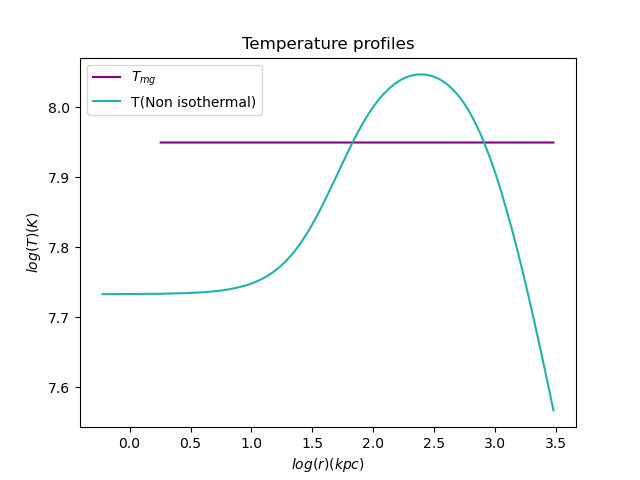
\includegraphics[width=12 cm]{temp1}
\caption{Comparison between the isothermal and non isothermal profile}
\label{fig:figure3}
\end{figure}

\begin{figure}
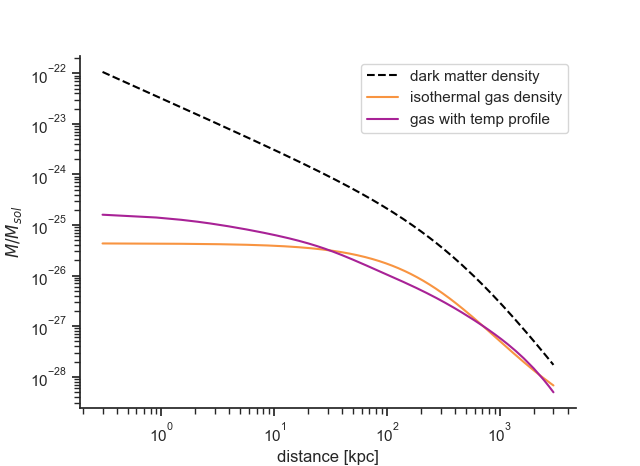
\includegraphics[width=0.8\textwidth, trim = 0 0 0 30]{gas1.png}
\caption{Comparison between the density profiles in the isothermal, no BGC regime and the non isothermal profile in presence of the BCG}
\label{fig:figure4}

\end{figure}



\newpage
\section{Diffusion of Fe in the ICM}
As a model for our cluster, we choose the Perseus Cluster: this problem involves solving the diffusion equation for the iron density \(\rho_{Fe}\), described in the following treatise. 

\subsection{Comparison with the work by Rebusco et al. }
The problem of diffusion of metals in the Perseus Cluster was approached in Rebusco et al. 2005, 2006; we take the observed abundance profile from their work, coming from XMM–Newton data (Churazov et al. 2003):
\begin{equation}
a(r)=Z_{Fe}(r)=0.3\frac{2.2+(r/80)^{3}}{1+(r/80)^{3}}a\odot .
\end{equation}
For the initial gas density, we use the one previously computed in the nonisothermal model in presence of the BCG. Its value is different from the one in Rebusco et al., which is: \(\rho_{0}=1.937 \cdot 10^{-24}n_{e}\; g/cm^{3},\) where \(n_{e}\) is the electron number density. \\
The difference between the Rebusco density profile and ours is plotted in Figure \ref{fig:figure5}. \\


\begin{figure}
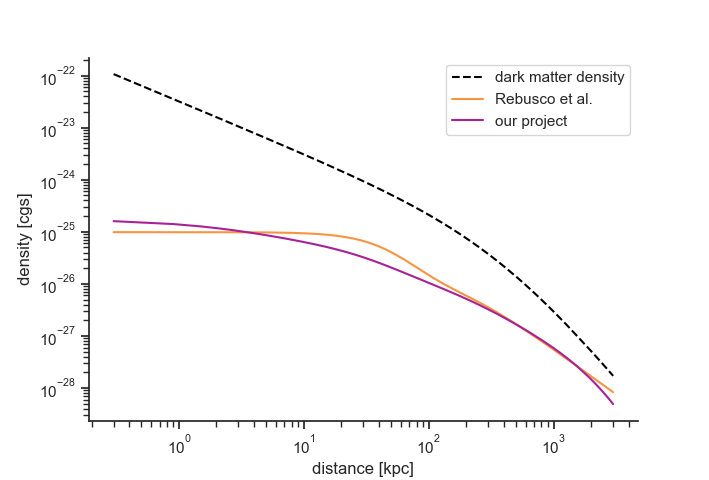
\includegraphics[hb,width=0.8\textwidth]{rebusco.png}
\caption{Comparison between the density profiles in our project and the one in Rebusco et al.}
\label{fig:figure5}
\end{figure}
Also, the temperature profile is different: in Rebusco et al. is described by: 
\begin{equation}
T(r)=7 \cdot \frac{1+(r/71)^{3}}{2.3+(r/71)^{3}} keV
\end{equation}
Again, the comparison with our model is plotted in Figure \ref{fig:figure6}.
\begin{figure}
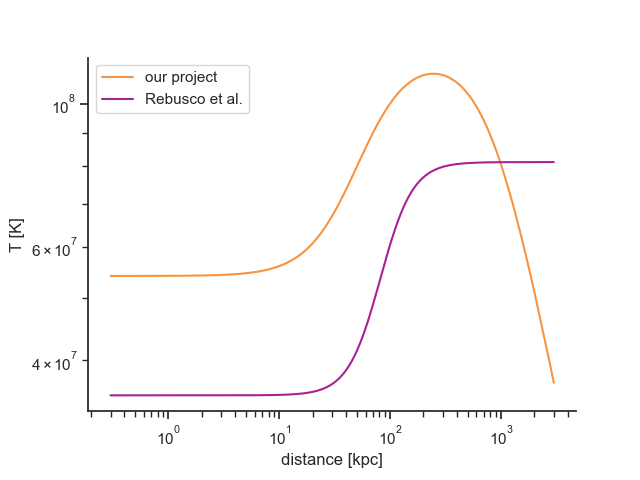
\includegraphics[width=0.8\textwidth]{temp2}
\caption{Comparison between the temperature profiles in our project and the one in Rebusco et al.}
\label{fig:figure6}
\end{figure}
%---------------------------------------------------------------------------------------------------------------------------
\subsection{Iron diffusion equation}
The equation describing the Iron diffusion is:

\begin{equation}
 %\frac{\partial f}{\partial t} = D \frac{\partial^2 f}{\partial x^2} + S
\frac{\partial na}{\partial t}= \nabla \cdot (Dn\nabla a) + S, \label{eq:diffusion1}
\end{equation}

where \(n=n(r)\) is the gas density, \(a=a(r,t)\) is the iron abundance, \(S=S(r,t)\) is the source term due to the iron injection from the BCG, and \(D\) is the diffusion coefficient.\\ Is a parabolic partial differential equation. As for project 1, a finite differences scheme is applied. This time no advection is present, which allows us to use a more simple resolutive scheme. more precisely we use explicit FTCS scheme.%that gave us a solution in the form:
%%%
%\begin{equation}
 %   f^{n+1}_i = f^n _i - \frac{D \Delta t}{\Delta x^2}(f^n _{i+1} - 2f^n_i +f^n_{i-1}) 
%\end{equation}
%%%
The turbulent diffusion coefficient can be approximated as \(D\approx v_{t}l_{t},\) where \(v_{t}\) is the typical turbulent velocity and \(l_{t}\) s the typical turbulence length-scale.\\
Equation \ref{eq:diffusion1} can be written as:

\begin{equation}
\frac{\partial \rho_{Fe}}{\partial t}= \frac{1}{1.4}\frac{1}{r^{2}}\frac{\partial(r^{2}D\rho \frac{\partial Z_{Fe}}{\partial r})}{\partial r} + S_{Fe}(r,t),
\end{equation}

where
\begin{equation}
Z_{Fe}=\frac{1}{1.4}\frac{\rho_{Fe}}{\rho}
\end{equation}
We see that, in order to solve the equation, we must know: the total gas density \(\rho(r)\), the diffusion coefficient \(D(r)\), and the initial iron abundance \(Z_{Fe}(r).\)\\
As initial conditions for \(\rho_{Fe}(r)\) and \(Z_{Fe}(r)\) we can use the profiles quoted in Rebusco et al., or alternatively we can start assuming \(Z_{Fe}(r)=0\) as the initial value and study the evolution including also the source term.\\


\textbf{Stability condition:} in order for the numerical scheme to be stable a limit on the value for the time step is requiered:
\begin{equation*}
    \Delta t \leq \frac{\Delta x^2}{2 D}
\end{equation*}
Since both $D$ and $\Delta x$ are constant, $\Delta t$ does not need to be calculated at each time step (unlike in project 1).


\newpage
\subsection{Preliminary results for only the diffusion term}
Here we only focus on the diffusion term. As initial condition, we took the Fe distribution observed in the Perseus cluster, with the background abundance subtracted. We then let the system evolve accordingly to the diffusion equation only:
\[
\frac{\partial \rho_{Fe}}{\partial t}=\frac{1}{1.4}\frac{1}{r^{2}}\frac{\partial(r^{2}D\rho \frac{\partial Z_{Fe}}{\partial r})}{\partial r}=\frac{1}{1.4}\frac{1}{r^{2}}\frac{\partial f(\rho_{Fe})}{\partial r},
\]
where we assume \(D\) and \(\rho(r)\) to be constant over time. the finite differences equation that we solve is:

\begin{equation}
    \rho^{n+1}_{Fe,j+\frac{1}{2}} =  \rho^{n}_{Fe,j+\frac{1}{2}} + \frac{\Delta t}{1.4}.\frac{[(r^2D\rho.\nabla_{Fe})^n_{j+1}-(r^2D\rho.\nabla_{Fe})^n_{j+1}]}{(r^3_{j+1}-r^3_{j})/3}
\end{equation}

Where:
\begin{equation}
   \nabla_{Fe,j}^n = \frac{Z^n_{Fe,j+1/2}-Z^n_{Fe,j-1/2}}{r_{j+1/2}-r_{j-1/2}}
\end{equation}

Notice the centering of the variable.\\

Results can be seen in fig \ref{fig:figure 7}. Before the time integration began, the total Fe mass in the grid is around $1.5129.10^{8}$ solar masses. After the diffusion (for 10 Gyr) we can see that the total mass is $1.5130.10^{8}$
solar masses. Of course some numerical errors are present, but still we are fine with the precision reached by our computations.
\begin{figure}[ht]
 \begin{minipage}[b]{8cm}
   
   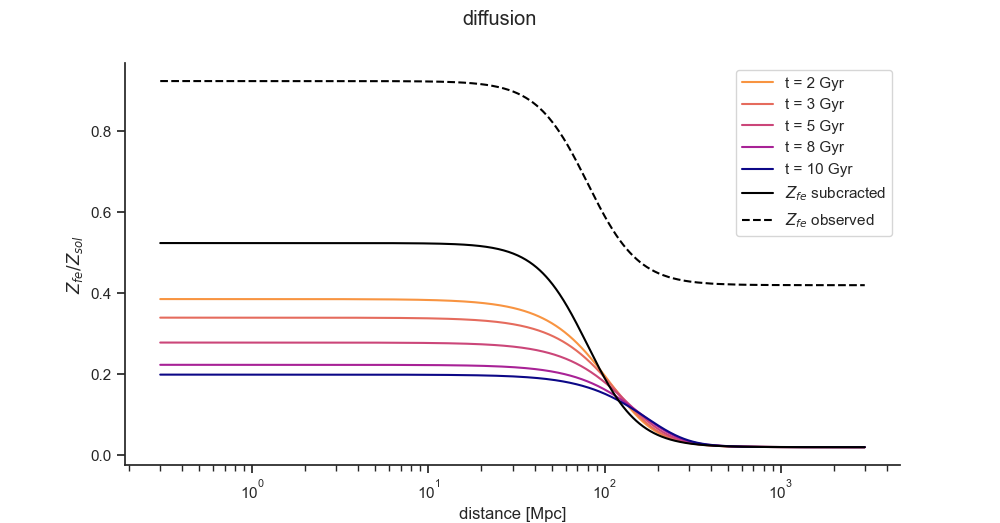
\includegraphics[trim = 0 0 0 10,width=16cm]{Figure_1.png}
   \caption{Result in the case of only diffusion}
   \label{fig:figure 7}
 \end{minipage}
 \ \hspace{2mm} \hspace{1mm} \
\end{figure}

\newpage
\subsection{Preliminary results for only the source term}
We have seen that we have two possible choices for the initial conditions on \(Z_{Fe}:\) either we can use the observed iron abundance in Perseus and check if the diffusion in presence of the BCG maintains that profile.  \\
Or we can take as initial condition $Z_{Fe} = 0$, and we seek to understand the behavior of our source term alone.
It must be known that our generic source term takes into account the contribution from:\\
a) type Ia SNe: each SNIa injects in the ICM a total mass of \(\sim 1.4 M_{\odot}\) and an iron mass \(\sim 0.74 M_{\odot};\)\\
b) stellar winds.\\
Both of these two events depend on the stellar density
\begin{equation*}
   \rho_{\star}(r)=\frac{M_{BCG}}{2\pi}\frac{a}{r}\frac{1}{(r+a)^{3}}. 
\end{equation*}
 
The term can approximately be written as: 
\begin{equation}
S_{Fe}(r)\simeq \rho_{\star}(r)[6.7\times 10^{-23}+3.13\times 10^{-20} \cdot SN_{rate}] \hspace{1cm} [gr.cm^{-3}.s^{-1}]
\end{equation}
Where the first term inside the brackets accounts for stellar winds, while the second one represents the injection by supernovas, and is obtained by a constant factor, times the supernova rate. \\ Here we assume a constant supernova rate of 0.015 $SN/s$.\\
This means that at each time cycle the source term injects a total amount of metals of the order of:

\begin{equation*}
    \rho^{n+1}_j = \rho^{n}_j + \Delta t . S_{Fe,j}
\end{equation*}
The Iron abundance is calculated accordingly eq 18. After 10 Gyr our source term has injected $1.1809.10^{8}$ solar masses of Fe. Compared with the total Fe mass observed, this source term alone cannot inject the right amount of iron into the ICM.

\begin{figure}[ht]
 \begin{minipage}[b]{8cm}
   
   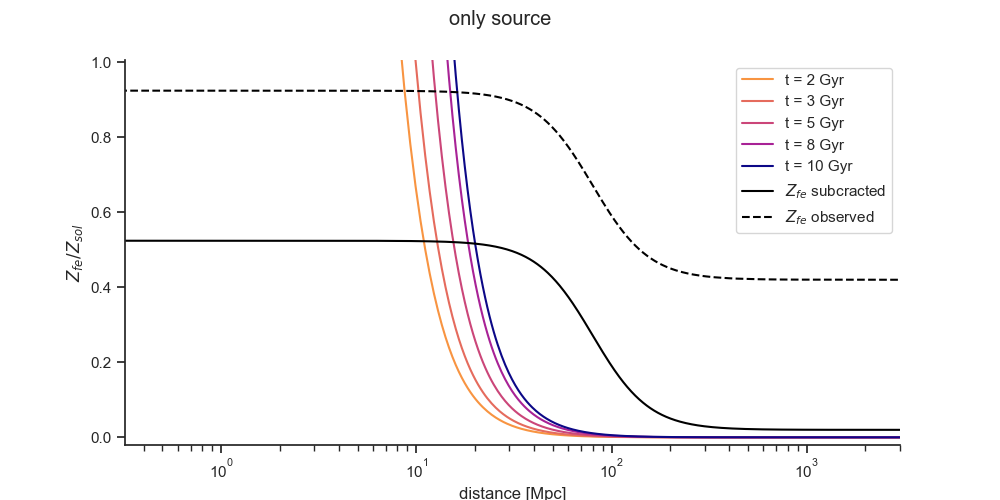
\includegraphics[trim= 0 0 0 12,width=15.7cm]{sorgente.png}
   \caption{Results in the case of only the source term}
 \end{minipage}
 \ \hspace{2mm} \hspace{1mm} \
\end{figure}

\newpage



\section{Results with the diffusion and source terms}
Finally, we consider both the contributions of the diffusion and source.\\ This is still a preliminary result since we already noted that the source term (as we wrote it) could not reproduce our observations.\\ Even more important is the effect of diffusion. in fig 10 is clear that our constant diffusion term spread the iron too smoothly and can not reproduce the step-like gradient we observe at around 90 Kpc.\\ This is even more clear if we allow the simulation to run up to 25 Gyr (much more than the Hubble time!), this extreme case is represented by the green line in fig 10. The general shape of the diffuse metals does not changes (of course, we just increase the time without modifying anything else), but the comparison with the observation is more clear: there are no possibilities for our simulation, in this stage, to agree with the observations.\\ We need to change our physical parameters such as; the source term and the diffusion coefficient.



\begin{figure}[ht]
 \begin{minipage}[b]{8cm}
   
   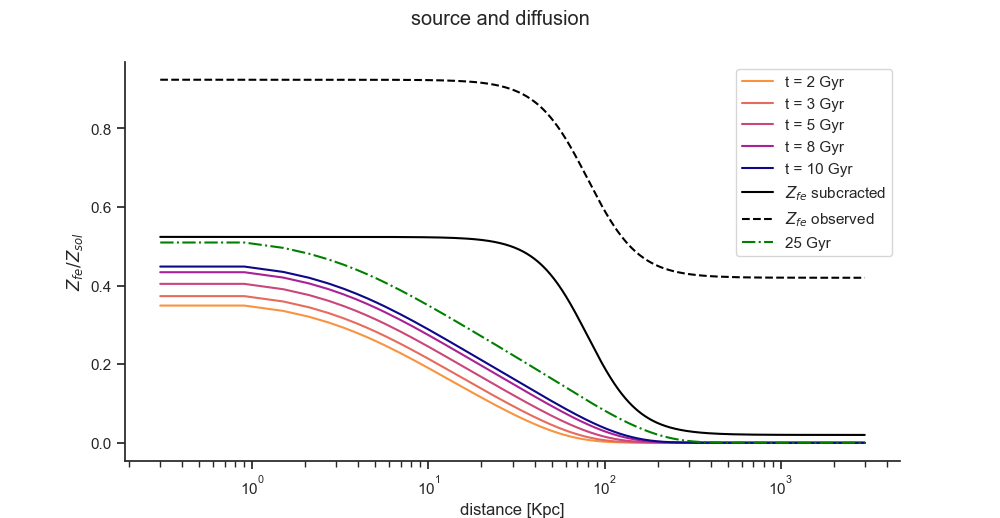
\includegraphics[trim = 0 0 0 0,width=16cm]{diff_sorg.png}
   %\caption{Prima figura}
 \end{minipage}
 \ \hspace{2mm} \hspace{1mm} \
\end{figure}


\subsection{Results with variable supernova rate}
As a final step, we decided to modify some physical parameters to (try to) better reproduce the observations. \\  More precisely we change the diffusion term $D$ and the supernova rate in eq 21, thus, making them no more constant. Now $SN_{rate}$ changes accordingly to the following time relation:

\begin{equation}
    SN_{rate} = 0.02*(\frac{t}{t_{now}})^{-1.1}
\end{equation}
The behavior of this equation shows a clear peak when $t << t_{now}$, with a power law decline for $t \rightarrow t_{mow}$.\\ This should approximate the real history of the supernova rate for the BCG, as discussed in the introduction.\\ Aside from the supernova rate, we also changed the diffusion coefficient. After experimenting with time-dependent $D$s, and grid-dependent $D$s, we opted for a more simple 2-values $D$. Not only it gives us the best agreements, but also (and most importantly), by being the simplest one, it's easier to justify in a more physical contest.   
\begin{equation*}
    D = \begin{cases} 9.95\cdot 10^{28}, & \mbox{if } r <\mbox{ 40} \mbox{Kpc}\\ 
        1.15\cdot 10^{29}, & \mbox{if } r >\mbox{ 40} \mbox{Kpc}
\end{cases}
\end{equation*}

Results are here represented; The burst in star formation that happens when the galaxy is still young, and the consequent high $SN_{rate}$, generates a huge amount of Fe in a very short time. This time is not long enough to allow the iron to diffuse over a few tens of Kpc and so a peak of very high metallicity is formed.\\ As time passes, the Fe abundance in the central region starts to drop, the fact that we assumed a slower diffusion time-scale near the BCG allows for a greater diffusion near 90 Kpc, and at the same time, does not let too much metals escape the central region. This should generate the step-like gradient we observe. \\ If we observe our result, we can say that for t=5 Gyr the gradient is very well reproduced, but the abundance in the central region is still too high. For t=8 Gyr instead, we face the opposite case, the quantity of Fe inside a radius of 40 Kpc is very good, but they are been spread in such a manner that the main feature of the gradient we seek to reproduce has been smoothed out by the diffusion. \\  The most plausible case should be an intermediate time, between 5 and 8 Gyr, most likely with a more realistic diffusion coefficient. In general is not wrong to imagine that, from the obtained results, the diffusion of Fe in the Perseus cluster, is likely regulated by a general diffusion coefficient of the order of $10^{29}$, While most of this iron has been injected around 8 or 7 Gyr ago. 

\begin{figure}[ht]
 \begin{minipage}[b]{8cm}
   
   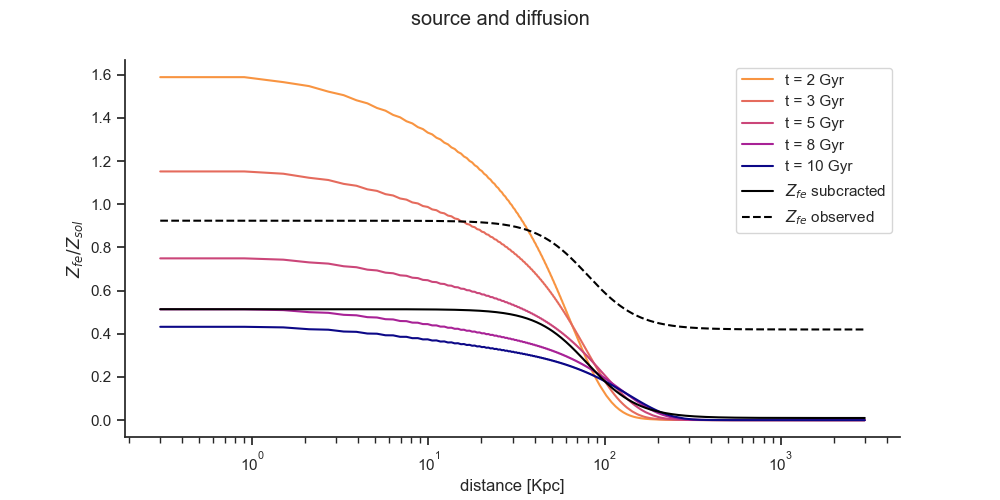
\includegraphics[trim = 0 0 0 0,width=16cm]{kappa.png}
   %\caption{Prima figura}
 \end{minipage}
 \ \hspace{2mm} \hspace{1mm} \
\end{figure}

\end{document}
